\chapter{Generating Encounters}
\label{chapter04}

We approach generating encounters as a search based problems with two different
approaches, Simulated Annealing \citep{ai-modern} and Evolution Strategies
\citep{evolution-strategies}.

To make the search algorithms as general as possible, we serialize our
internal game representation into a single vector of normalized floating
point values (DNA). The algorithm then doesn't need to understand our game
mechanics and restriction, and can be applied to different configurations of
the game independently.

To avoid balancing via specific attributes, one can simply remove them from
the serialization/deserialization routines that transform the game setup into
the DNA vector, without altering any of the logic for balancing encounters.

In the case of our experiments, we chose to stick with 2v2 games on a fixed map,
where each mage has only two abilities. This was chosen both with respect to our
questionnaire, and running time of the algorithms. Choosing a larger team setup or
a bigger map (or many different maps) would be difficult for the participants,
and would also take much longer to compute our experimental data.

Taking these restrictions into mind, the DNA would then take up $96$ floating point values,
specifically: $$2 \text{ Teams} \times 2 \text{ Mages} \times ( HP + AP + \text{ AbilitySize})$$ where $\text{Ability Size} = 11$ since we need to serialize damage, cost, range, cooldown,
debuff (HP damage, AP damage, lifetime), and AOE (debuff + lifetime).

\section{Simulated Annealing and Evolution Strategies}

Our initial implementation of generating the encounters was using Simulated
Annealing. However, we had difficulty converging to good results \todo{fuj,
napsat jinak}.

As a result, we ran an experiment to sample the search space at roughly 20
million different points, and measured the change in fitness in the
neighbourhood of each point. We found that in each point's neighbourhood,
there are roughly 5 times more points that have worse fitness than the ones
that are an improvement over the current point. We also found that most of
these downward changes were much steeper between 4--7x than the improving
points. Our suspicion is that this is the main cause of failure of
Simmulated Annealing, which simply fails to find the upward slope.

For this reason we chose to try another approach, specificially Evolution
Strategies. In short, we take the initial DNA vector, generate around 50
neighbours in the search space, evaluate their fitness and take their weighted
sum as the new current DNA\@. This process is iterated until a DNA with
suitable fitness is found. We have found this approach to consistently converge
much faster than simulated annealing.

\section{Choice of the Fitness Function}

In order to evaluate the balance of a matchup, we evaluated the following three
criteria:

\begin{description}
\item [Balance] Unsurprisingly, part of the fitness function is comparing the strength of both teams against each other.
\item [Game length] We also put an interval restriction on game length.
\item [Team difference] Lastly, since we don't to create balance by making both teams identical, we added a third criteria
that measures the difference of both teams.
\end{description}

The combined fitness function is calculated as the average of the three. See \hyperref[fig:converging-es]{Figure 4.1} for an example
plot of how the fitness function converges using Evolution Strategies.

\begin{figure}
	\centering
	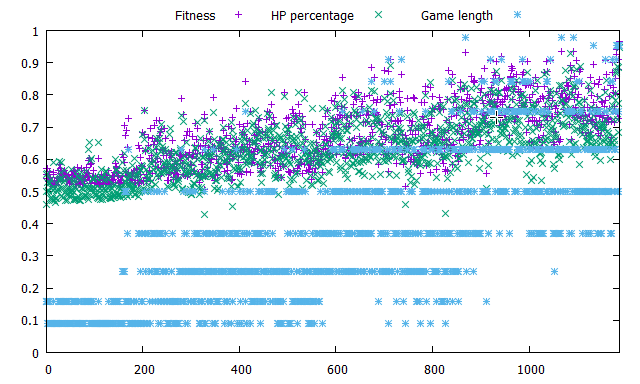
\includegraphics[width=0.75\textwidth]{img/converging-es.png}
	\caption{An exmple of a how the combined fitness function converges over rougly 1200 iterations. Green dots represent the \emph{Balance} fitness measuring HP percentage left at the end of the game, blue dots represent game length, and purple is the combined fitness. We're not showing team difference data points as in this plot.}
	\label{fig:converging-es}	
\end{figure}

\todo{tady neco chybi, prijde mi, ze to nenavazuje}

During the experiment we encountered multiple ways ES tried to exploit the
game mechanics to maximize the balance fitness function in ways that were
undesirable. One example being when the resulting games end up being short
as the algorithm generates mages with lots of AOE abilities that cover the
whole map in the first turn, resulting in immediate death of all characters.

We balance this by introducing an additional fitness function for game length
in the form of a cumulative normal distribution with mean around $10$ turns.

Lastly, the team difference is measured as an euclidean distance between the DNA
vectors of each team. Again, we use a cumulative normal distribution to put a lower
bound on the team difference.
